\section{Motion Estimation and Video Coding}


\begin{questionbox}{Domanda 74}
\textbf{Motion estimation}: give the principles of the block matching approach. Give at least one cost function. [Bonus]. Discuss the regularization issue.
\end{questionbox}


\begin{itemize}
  \item \textbf{Block matching} $\rightarrow$ split frame into blocks $B_{p,q}$; search similar block in reference frame window.
  \item \textbf{Best displacement}:

\end{itemize}
$$
(\hat{i},\hat{j})=\arg\min_{(i,j)\in W}J(i,j)
$$

\begin{itemize}
  \item \textbf{SSD}:

\end{itemize}
$$
J_{\text{SSD}}(i,j)=
\sum_{(n,m)\in B_{p,q}}
[f(n,m,k)-f(n-i,m-j,h)]^2
$$

\begin{itemize}
  \item \textbf{SAD}:

\end{itemize}
$$
J_{\text{SAD}}(i,j)=
\sum_{(n,m)\in B_{p,q}}
|f(n,m,k)-f(n-i,m-j,h)|
$$

\begin{itemize}
  \item \textbf{Regularized}:

\end{itemize}
$$
J_{\text{REG}}(i,j)=
\|\vec{f}_k(B_{p,q})-\vec{f}_h(B_{p-i,q-j})\|_p^p
+\lambda R(i,j)
$$

\begin{itemize}
  \item \textbf{Regularization} $\rightarrow$ penalizes expensive/irregular motion vectors; balances prediction quality with motion-vector coding rate.

\end{itemize}
\begin{questionbox}{Domanda 75}
Discuss the advantages and the disadvantages of Intra, Predictive, and Bidirectional images in a GOP for video coding.
\end{questionbox}


\begin{itemize}
  \item \textbf{I images}:
  \begin{itemize}
    \item intra only;
    \item \textbf{advantages} $\rightarrow$ random access, error reset, no motion estimation;
    \item \textbf{disadvantages} $\rightarrow$ high rate, lower compression.
  \end{itemize}
  \item \textbf{P images}:
  \begin{itemize}
    \item predicted from previous anchor frames;
    \item \textbf{advantages} $\rightarrow$ good compression, moderate delay;
    \item \textbf{disadvantages} $\rightarrow$ ME/MC complexity, error propagation.
  \end{itemize}
  \item \textbf{B images}:
  \begin{itemize}
    \item predicted from past and future frames;
    \item \textbf{advantages} $\rightarrow$ best compression;
    \item \textbf{disadvantages} $\rightarrow$ highest complexity, structural delay, not ideal for low latency.
  \end{itemize}
  \item GOP structure controls compression efficiency, delay, random access interval, error propagation.

\end{itemize}
\begin{questionbox}{Domanda 76}
(ME) Describe the dif and only iference between “motion field” and “optical flow”.
\end{questionbox}


\begin{itemize}
  \item \textbf{Motion field} $\rightarrow$ projection of actual 3D scene motion onto image plane.
  \item \textbf{Optical flow} $\rightarrow$ apparent motion of brightness patterns.
  \item They often coincide, but can dif and only ifer due to illumination changes, occlusions, texture ambiguities.

\end{itemize}
\begin{questionbox}{Domanda 77}
(ME) Explain the Horn and Schunck algorithm’s core principle for dense optical flow estimation.
\end{questionbox}


\begin{itemize}
  \item \textbf{Optical flow constraint}:

\end{itemize}
$$
u f_x + v f_y + f_t = 0
$$

\begin{itemize}
  \item \textbf{Horn-Schunck objective}:

\end{itemize}
$$
J=
\iint_{\mathcal{R}}(u f_x+v f_y+f_t)^2\,dxdy
+\lambda\iint_{\mathcal{R}}(\|\nabla u\|^2+\|\nabla v\|^2)\,dxdy
$$

\begin{itemize}
  \item \textbf{First term} $\rightarrow$ brightness consistency.
  \item \textbf{Second term} $\rightarrow$ smooth dense flow field.

\end{itemize}
\begin{questionbox}{Domanda 78}
(ME) Discuss the Rate-Distortion trade-off when selecting block sizes in motion estimation.
\end{questionbox}


$$
J(v)=d(B_k^{(p)},B_h^{(p+v)})+\lambda_{ME}R(v)
$$

\begin{itemize}
  \item \textbf{Large blocks}:
  \begin{itemize}
    \item fewer motion vectors;
    \item lower side information and complexity;
    \item worse fit near object boundaries.
  \end{itemize}
  \item \textbf{Small blocks}:
  \begin{itemize}
    \item better prediction and lower distortion;
    \item more motion vectors and partition bits;
    \item higher complexity.

  \end{itemize}
\end{itemize}
\begin{questionbox}{Domanda 79}
(ME) Which of the following is a disadvantage of using the Sum of Squared Dif and only iferences (SSD) as a matching criterion?
\end{questionbox}


\begin{itemize}
  \item \textbf{SSD squares errors} $\rightarrow$ outliers dominate cost.
  \item Illumination changes, noise, occlusions $\rightarrow$ irregular motion vectors.
  \item \textbf{SAD} $\rightarrow$ often more robust and cheaper.

\end{itemize}
\begin{questionbox}{Domanda 80}
(ME) What is the main benefit of the Hexagon Search strategy compared to Full Search?
\end{questionbox}


\begin{itemize}
  \item \textbf{Full search} $\rightarrow$ tests all candidates; optimal within window, expensive.
  \item \textbf{Hexagon search} $\rightarrow$ tests small hexagonal pattern iteratively; far fewer evaluations.
  \item \textbf{Benefit} $\rightarrow$ faster search.
  \item \textbf{Cost} $\rightarrow$ no guaranteed global optimum.

\end{itemize}
\begin{questionbox}{Domanda 81}
(ME) What does an affine motion model allow that a pure translational model does not?
\end{questionbox}


\begin{itemize}
  \item \textbf{Translation} $\rightarrow$ constant displacement only.
  \item \textbf{Affine motion} $\rightarrow$ rotation, zoom, shear:

\end{itemize}
$$
\vec{v}(p)=\vec{b}+Bp
=
\begin{bmatrix}b_1\\b_2\end{bmatrix}
+
\begin{bmatrix}b_3&b_4\\b_5&b_6\end{bmatrix}p
$$

\begin{itemize}
  \item If $B=0$ $\rightarrow$ pure translation / block matching.

\end{itemize}
\begin{questionbox}{Domanda 82}
Draw the block diagram of a hybrid video encoder (motion estimation/compensation + DCT + quantization + entropy coding + reconstruction loop with frame buffer). Explain why the encoder contains an internal decoder.
\end{questionbox}


\begin{itemize}
  \item \textbf{Hybrid video encoder} $\rightarrow$ codes prediction residual, usually not whole frame.

\end{itemize}
\begin{figure}[H]
\centering
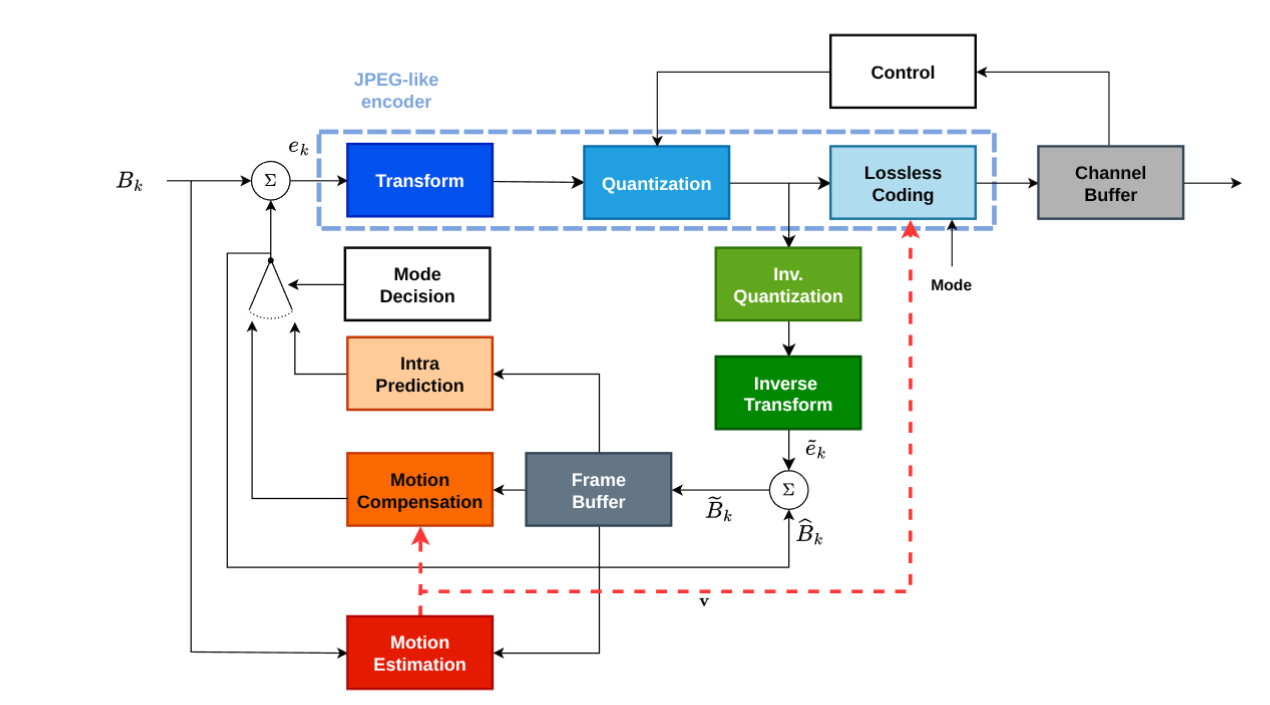
\includegraphics[width=0.75\textwidth]{images/Hybrid_video_encoder.png}
\caption{Hybrid video encoder.png}
\end{figure}

\begin{itemize}
  \item \textbf{Mode decision} $\rightarrow$ selects intra/inter predictor.
  \item \textbf{Transform + quantization} $\rightarrow$ residual coding.
  \item \textbf{Lossless coding} $\rightarrow$ bitstream.
  \item Inverse quantization + inverse transform $\rightarrow$ reconstructed residual.
  \item \textbf{Reconstructed block} $\rightarrow$ frame buffer for later motion compensation.
  \item \textbf{Internal decoder needed} $\rightarrow$ future predictions must use same reconstructed frames as decoder; otherwise drift propagates.

\end{itemize}
\begin{questionbox}{Domanda 83}
(VCP) Why is the temporal prediction error usually more efficient to encode than the original video signal?
\end{questionbox}


\begin{figure}[H]
\centering
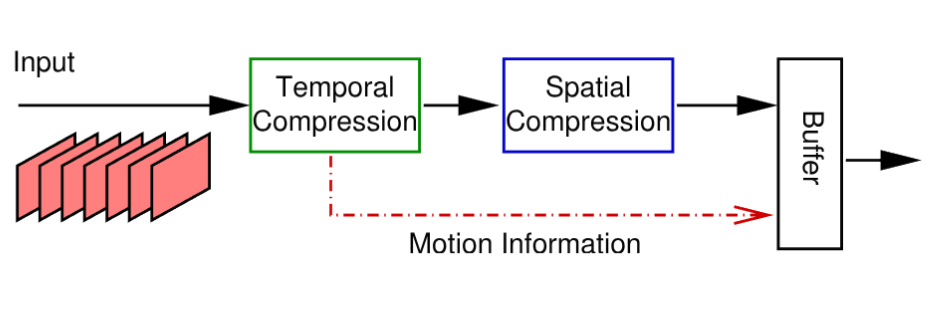
\includegraphics[width=0.75\textwidth]{images/Video_coding_principles.png}
\caption{Video coding principles.png}
\end{figure}

\begin{itemize}
  \item \textbf{Video frames} $\rightarrow$ highly correlated.
  \item Motion-compensated prediction estimates current block from reference frames.
  \item \textbf{Encode only residual}:

\end{itemize}
$$
e=x-x_p
$$

\begin{itemize}
  \item \textbf{Residual} $\rightarrow$ lower energy and more sparse than original frame.
  \item \textbf{Consequence} $\rightarrow$ transform quantization and entropy coding more efficient.

\end{itemize}
\begin{questionbox}{Domanda 84}
(VCP) Describe the function of the “Mode Selection” step in a hybrid video encoder.
\end{questionbox}


\begin{itemize}
  \item \textbf{Mode selection} $\rightarrow$ choose coding mode minimizing R-D cost:

\end{itemize}
$$
J = D+\lambda R
$$

\begin{itemize}
  \item \textbf{For blocks}:

\end{itemize}
$$
D=\sum_{k=1}^{K}D_k(i_k,Q),
\quad
R=\sum_{k=1}^{K}R_k(i_k,Q)
$$

$$
J(\vec{i},Q,\lambda)=D(\vec{i},Q)+\lambda R(\vec{i},Q)
$$

\begin{itemize}
  \item \textbf{Block-wise suboptimal minimization}:

\end{itemize}
$$
i_k^\star=\arg\min_{i_k}J_k(i_k,Q,\lambda)
$$

\begin{itemize}
  \item \textbf{Empirical choices}:

\end{itemize}
$$
\text{MPEG-2: } \lambda=aQ^2+b
$$

$$
\text{H.264: } \lambda=c\cdot2^{dQ+e},
\quad
\lambda_{ME}=\sqrt{\lambda}
$$

\begin{questionbox}{Domanda 85}
(VCP) How does the “Channel Buffer” controller manage the trade-off between target rate and video quality?
\end{questionbox}


\begin{itemize}
  \item \textbf{Channel buffer} $\rightarrow$ controls quantization step to meet target rate.
  \item \textbf{Buffer occupancy high} $\rightarrow$ increase quantization step $\rightarrow$ reduce rate, lower quality.
  \item \textbf{Buffer occupancy low} $\rightarrow$ decrease quantization step $\rightarrow$ improve quality, higher rate.
  \item \textbf{Goal} $\rightarrow$ avoid overflow/underflow while keeping quality high.

\end{itemize}
\begin{questionbox}{Domanda 86}
(VCP) What is the primary role of an “I-frame” in a GOP structure?
\end{questionbox}


\begin{itemize}
  \item \textbf{I-frame} $\rightarrow$ intra-coded and independently decodable.
  \item \textbf{Roles} $\rightarrow$ random access, GOP start, temporal error-propagation limit.

\end{itemize}
\begin{questionbox}{Domanda 87}
(VCP) In the context of motion vector coding, why is a Median Predictor (MVP) used?
\end{questionbox}


\begin{itemize}
  \item \textbf{Neighboring motion vectors} $\rightarrow$ correlated.
  \item Median predictor estimates current vector from adjacent blocks.
  \item \textbf{Encoder sends only dif and only iference}:

\end{itemize}
$$
\text{MVD} = \text{MV} - \text{MVP}
$$

\begin{itemize}
  \item \textbf{MVD usually small} $\rightarrow$ cheaper to encode.

\end{itemize}
\begin{questionbox}{Domanda 88}
(VCP) What happens in the decoder when it receives an “Inter-coded” block?
\end{questionbox}


\begin{figure}[H]
\centering
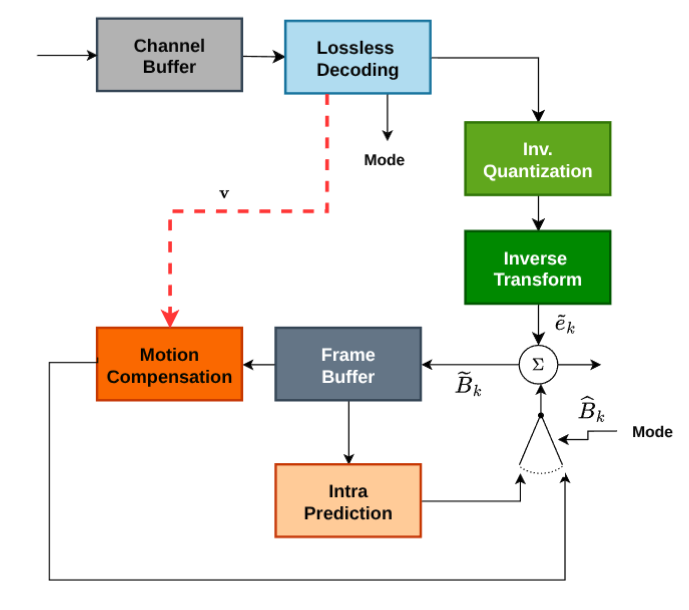
\includegraphics[width=0.75\textwidth]{images/Hybrid_video_decoder.png}
\caption{Hybrid video decoder.png}
\end{figure}

\begin{itemize}
  \item \textbf{Decoder reads side information} $\rightarrow$ mode, reference index, motion vector.
  \item \textbf{Entropy decoding} $\rightarrow$ residual and side information.
  \item Inverse quantization + inverse transform $\rightarrow$ reconstructed residual.
  \item Motion compensation / intra prediction $\rightarrow$ predictor.
  \item \textbf{Reconstruction}:

\end{itemize}
$$
\hat{x}=\text{prediction}+\hat{e}
$$

\begin{itemize}
  \item Output stored in frame buffer.

\end{itemize}
---

